\subsubsection{Unterschiede zur Referenzimplementierung}
\label{bpr:effizienz:modifikationen}

Die Implementierung des \bpr Algorithmus für das \sacabench Framework erfolgte in erster Linie entlang der im Paper \cite{saca:2} beschriebenen Variante des Algorithmus. Daraus ergaben sich zunächst einige strukturelle Unterschiede des Quellcodes im Vergleich zur Referenzimplementierung des Autors. Erst nach der Fertigstellung einer lauffähigen und stabilen Implementierung wurden dann die von Schürmann beschriebenen Modifikationen \cite[Kapitel 3]{saca:2} implementiert, die zur Verbesserung der praktischen Laufzeit beitragen sollen, ohne die asymptotische Laufzeit zu beeinflussen.\par
Erst im Anschluss daran fand ein direkter Vergleich der beiden Implementierungen statt, der einige algorithmische Unterschiede in der Umsetzung von Teilfunktionen offenbarte. Teilweise konnte die Laufzeit durch Anpassung derartiger Codestellen an das Original verringert werden, während sich in anderen Funktionen die neu implementierte Variante als effizienter herausstellte. In allen Fällen wurde dann jeweils die schnellere Methode beibehalten. Die wichtigsten dadurch entstandenen Unterschiede zwischen der Referenzimplementierung und derer der Projektgruppe werden in diesem Kapitel aufgeführt.

\paragraph{Seward's copy}
\label{bpr:seward}
Beide Varianten des Algorithmus verwenden die von Seward \cite{seward2000} beschriebene Copy-Technik, um aus bereits sortierten Einträgen die Reihenfolge von bis dahin unsortierten Suffixen abzuleiten. 
\begin{figure}[ht]
	\resizebox{\textwidth}{!}{
		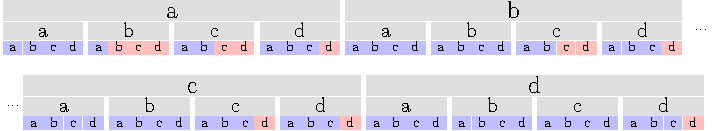
\includegraphics{kapitel/saca_algorithmen/bpr/effizienz/modifikationen/seward/image.pdf}
	}
    \caption[Funktionsweise der Copy-Technik]{Level-1 bis Level-3 Buckets über dem Alphabet \(\{a, b, c, d\}\). Rot markierte Buckets müssen mit Quicksort sortiert werden. Blau markierte Buckets können in Linearzeit induziert werden.}
	\label{fig:seward}
\end{figure}
Der Unterschied besteht lediglich in der Reihenfolge, in der die Sortieroperationen und das Induzieren angewendet werden: Während Schürmann nach jedem Durchlauf durch einen Top-Level Bucket direkt den Rest dieses Buckets induziert und danach erneut die Bucket-Pointer aktualisiert, werden bei der \sacabench-Implementierung zuerst alle Top-Level Buckets vorsortiert, bevor im Anschluss in einem Durchlauf alle verbleibenden Indizes zusammen induziert werden. 
\begin{listing}[h]
    \begin{minipage}{0.5\textwidth}
        \begin{minted}[autogobble, mathescape]{python}
            # m is assumed to be $|\Sigma|$
            for x in 0..m-1
              for y in x+1..m-1
                for z in y..m-1
                  quicksort on bucket xyz
                  update bucket pointers
            for x in 0..m
              seward-copy rest of bucket x
        \end{minted}
    \end{minipage}
    \begin{minipage}{0.5\textwidth}
        \begin{minted}[autogobble, mathescape]{python}
            # m is assumed to be $|\Sigma|$
            for x in 0..m-1
              for y in x+1..m-1
                for z in y..m-1
                  quicksort on bucket xyz
                  update bucket pointers
              seward-copy rest of bucket x
              update bucket pointers
        \end{minted}
    \end{minipage}
    \caption[Verwendung der Copy Technik]{Verwendung der Copy Technik der \sacabench-Version (links) und bei Schürmann (rechts)}
\end{listing}
Letzteres erspart im Vergleich zur Referenzimplementierung die Aktualisierung der Bucket-Pointer nach dem Induzieren, welche als Random Access auf das Array einen messbaren Teil der Laufzeit verursachen. Die Aktualisierung kann weg fallen, da die Bucket-Pointer lediglich als Sortierschlüssel für Quicksort verwendet werden, was aber in dieser Variante zum Zeitpunkt der Induzierung schon abgeschlossen werden.\par
Zu erwarten ist, dass bedingt durch die zum Zeitpunkt der späteren Quicksort-Aufrufe im Vergleich zur Referenzimplentierung noch ungenaueren Sortierschlüssel mehr Sortieraufrufe durchgeführt werden müssen, was eine längere Laufzeit zur Folge hat. Ein solcher Effekt war jedoch für Eingabegrößen bis zu mehreren hundert Megabyte nicht messbar.

\paragraph{Adressierung der Arrays}
Die Referenzimplementierung von Schürmann verwendet für die Einträge im Suffixarray 64 Bit lange Zeiger auf die zugehörige Speicherstelle im Eingabetext, an der das jeweilige Suffix beginnt. Analog dazu werden im Bucket-Pointer Array \bptr 64 Bit lange Zeiger auf die Einträge im Suffixarray gespeichert. Alle Zugriffe auf diese Arrays finden über direkte Pointer-Arithmetik statt.\par
In der \sacabench-Implementierung des Algorithmus werden für alle Zugriffe auf Arrays durch Indexzugriffe durchgeführt. Das ermöglicht es, je nach Größe der Eingabe die Bitbreite für die Adressierung dynamisch festzulegen. Da für die meisten in annehmbarer Zeit zu verarbeitenden Eingaben eine Größe von 32 Bit ausreicht, kann in den meisten Fällen der Speicherbedarf sowohl für das Suffixarray als auch für das Bucket-Pointer Array halbiert werden. Dadurch halbiert sich (abgesehen von konstantem Zusatzspeicher) der gesamte Speicherbedarf des Algorithmus auf die Hälfte. Ein messbarer Unterschied in der Laufzeit hat sich dadurch jedoch nicht ergeben.

\paragraph{Sortieralgorithmus für Schlüssel}
In der Referenzimplementierung verwendet Schürmann eine Version von Quicksort, um die Suffixe innerhalb der Buckets anhand ihrer Schlüssel zu sortieren. Für kleine Buckets mit einer Größe von maximal 15 Elementen wird dort Insertionsort verwendet. Einen deutlichen Vorteil gegenüber den von uns getesteten Varianten von Quicksort bietet in den meisten Fällen der Algorithmus In-Place Parallel Super Scalar Samplesort (IPS\(^4\)o \cite{axtmann2017}). Die Verwendung dieses Algorithmus hat die tatsächliche Laufzeit auf natürlichsprachlichen Eingaben von über 50\,MB ausreichend beschleunigt, um eine schnellere Verarbeitung zu ermöglichen als die Referenzimplemtierung. Bei repetitiven Texten hingegen fällt der Vorteil von Quicksort und IPS\(^4\)o deutlich geringer aus. Ein Unterschied ist hier nicht mehr messbar.
